% ****** Start of file apssamp.tex ******
%
%   This file is part of the APS files in the REVTeX 4.1 distribution.
%   Version 4.1r of REVTeX, August 2010
%
%   Copyright (c) 2009, 2010 The American Physical Society.
%
%   See the REVTeX 4 README file for restrictions and more information.
%
% TeX'ing this file requires that you have AMS-LaTeX 2.0 installed
% as well as the rest of the prerequisites for REVTeX 4.1
%
% See the REVTeX 4 README file
% It also requires running BibTeX. The commands are as follows:
%
%  1)  latex apssamp.tex
%  2)  bibtex apssamp
%  3)  latex apssamp.tex
%  4)  latex apssamp.tex
%
\documentclass[
reprint,
superscriptaddress,
% groupedaddress,
amsmath,
amssymb,
aps,
% prl,
% showpacs,
%unsortedaddress,
%runinaddress,
%frontmatterverbose, 
%preprint,
%showpacs,preprintnumbers,
%nofootinbib,
%nobibnotes,
%bibnotes,
%pra,
%prb,
%rmp,
%prstab,
%prstper,
%floatfix,
]{revtex4-1}

\usepackage{graphicx}% Include figure files
\usepackage{dcolumn}% Align table columns on decimal point
\usepackage{bm}% bold math
\usepackage{amssymb}   % for math
\usepackage{hyperref}% add hypertext capabilities
\usepackage{aas_macros}
%\usepackage[mathlines]{lineno}% Enable numbering of text and display math
%\linenumbers\relax % Commence numbering lines

%\usepackage[showframe,%Uncomment any one of the following lines to test 
%%scale=0.7, marginratio={1:1, 2:3}, ignoreall,% default settings
%%text={7in,10in},centering,
%%margin=1.5in,
%%total={6.5in,8.75in}, top=1.2in, left=0.9in, includefoot,
%%height=10in,a5paper,hmargin={3cm,0.8in},
%]{geometry}

\begin{document}

\preprint{APS/123-QED}

\title{Detecting Cosmic Reionization using Novel Radio Interferometric Approach}% Force line breaks with \\
% \thanks{A footnote to the article title}%

\author{Nithyanandan Thyagarajan}
\email{t\_nithyanandan@nrao.edu}
\homepage{https://tnithyanandan.wordpress.com/}
\thanks{Nithyanandan Thyagarajan is a Jansky Fellow of the National Radio Astronomy Observatory.}
\affiliation{National Radio Astronomy Observatory, Socorro, NM 87801, USA}
% \altaffiliation[Also at ]{Physics Department, XYZ University.}%Lines break automatically or can be forced with \\
\author{Chris L. Carilli}%
% \email{Second.Author@institution.edu}
\affiliation{National Radio Astronomy Observatory, Socorro, NM 87801, USA}

% \collaboration{MUSO Collaboration}%\noaffiliation

\author{Bojan Nikolic}
% \homepage{http://www.Second.institution.edu/~Charlie.Author}
\affiliation{Astrophysics Group, Cavendish Laboratory, University of Cambridge, Cambridge CB3 0HE, UK}%
% \affiliation{
%  Third institution, the second for Charlie Author
% }%

% \collaboration{CLEO Collaboration}%\noaffiliation

\date{\today}% It is always \today, today,
             %  but any date may be explicitly specified

\begin{abstract}
Detecting neutral Hydrogen (H~{\sc i}) in the IGM at $z\gtrsim 6$ has been identified as a most direct and promising probe of cosmic dawn and the epoch of reionization (EoR) -- epochs that signify a major phase transition in the Universe. Current experiments have not lived up to the initial promise of high-significance detection of H~{\sc i} from these cosmic epochs because bright astrophysical foreground objects such as radio galaxies and the Milky Way, and ionospheric and instrumental effects overwhelm the cosmic signal by many orders of magnitude. Extracting the cosmological signal from such data necessitates extremely precise antenna calibration, a feat that has been very hard to achieve. We propose using the phase of the bi-spectrum from interferometric measurements to eliminate this requirement by making antenna-based calibration terms and ionospheric distortions irrelevant. This quantity is composed purely of information about the sky besides stochastic measurement noise and is thus uncontaminated by antenna characteristics and uncertainties therein. We show that the bi-spectrum phase of foreground emission has a characteristically smooth spectrum relative to the cosmological signal. Thus the latter can be separated effectively by exploiting this characteristic spectral difference using a Fourier-domain approach called the ``delay spectrum'', while eliminating the need for precise calibration of antennas altogether that would have been essential to account for phases introduced by the instrument and ionospheric propagation effects in current approaches. By removing this burden, our approach significantly advances the prospects of directly detecting these high-redshift cosmic epochs relative to current approaches. Give some numbers for the prospects for detection.
\end{abstract}

% \begin{abstract}
% An article usually includes an abstract, a concise summary of the work
% covered at length in the main body of the article. 
% \begin{description}
% \item[Usage]
% Secondary publications and information retrieval purposes.
% \item[PACS numbers]
% May be entered using the \verb+\pacs{#1}+ command.
% \item[Structure]
% You may use the \texttt{description} environment to structure your abstract;
% use the optional argument of the \verb+\item+ command to give the category of each item. 
% \end{description}
% \end{abstract}

\pacs{}% PACS, the Physics and Astronomy
                             % Classification Scheme.
%\keywords{Suggested keywords}%Use showkeys class option if keyword
                              %display desired

% \pacs{Valid PACS appear here}% PACS, the Physics and Astronomy
%                              % Classification Scheme.
% %\keywords{Suggested keywords}%Use showkeys class option if keyword
%                               %display desired

\maketitle

%\tableofcontents

\section{Introduction}\label{sec:intro}

One of the most pursued goals in modern astrophysics and cosmology is the characterization of the different phase transitions the Universe has undergone since the recombination era ($\sim 300,000$ years after the Big Bang, $z\approx 1100$). Since then the Universe remained predominantly neutral (known as the ``Dark Ages'') until the gravitational collapse around peaks in the primordial matter density fluctuations created the first astrophysical objects, namely, stars and galaxies ($\sim$ 200--400 million years after the Big Bang) that produced photons energetic enough to re-ionize the intergalactic medium around them. This epoch is known as ``cosmic dawn''. It evolved into the epoch of reionization (EoR), which signified a phase transition in the Universe where photon-to-baryon eventually exceeded unity making the entire Universe ionized again, marking the end of EoR ($\sim$ 1 billion years after Big Bang, or $z\gtrsim 6$). The astrophysical processes in these epochs shaped the evolution of gas and galaxy, and large-scale structure now observed in the local Universe. However, they are among the most poorly explored epochs in the Universe's history. The redshifted 21~cm spectral line from the spin-flip transition of electron spin in the neutral Hydrogen (H~{\sc i}) atom, the most abundant element in the Universe, promises to be most direct probe yet in filling gaps in our understanding of the Universe's history \cite{sun72,sco90,mad97,toz00,ili02,fan02,fan06,bar07,mor10}.

Our Galaxy and intervening radio galaxies in the foreground of the EoR signal produce synchrotron emission in the same band, which is expected to be orders of magnitude brighter than the latter. However, the synchrotron foregrounds have a smooth spectrum whereas the H~{sc i} signal from the EoR will appear as small fluctuations superimposed on the smooth foreground spectrum. The hope of separating the cosmic signal from the Galactic and extragalactic synchrotron foregrounds spawned a number of low-frequency instruments including the Precision Array for Probing the Epoch of Reionization (PAPER) \cite{par10}, the Murchison Widefield Array (MWA) \cite{tin13}, and the Low Frequency Array (LOFAR) \cite{van13} with sensitivity forecasts sufficient for a high-significance statistical detection of these EoR H~{\sc i} spectral fluctuations using power spectrum methodology with $\sim$ 1000 hours of observations \cite{bea13,thy13}. 

However, despite obtaining sufficient quantity of data, the challenges in these experiments such as spectral systematics in the precision of calibration \cite{barry16}, instrumental artifacts, wide-field effects \cite{thy15a,thy15b}, antenna beam chromaticity \cite{thy16}, reflections in geometrical and electrical paths \cite{thy16}, are further compounded by the extreme brightness of foregrounds and have thus limited the results to upper bounds on the strength of the signal \cite{pac13,ali15,patil17} and weak constraints on the astrophysical parameters \cite{pob15}. 

These experiments operate under the challenge of extreme dynamic range requirements $\gtrsim 10^4$ \cite{dim02,ali08,ber09,ber10,dat10,gho12}. Their success critically depends on highly precise and accurate calibration against departures from ideal behavior introduced by the complex instrument response and the ionosphere. Thus, the accuracy of instrument response and knowledge about the instrument and any models used in the analysis (e.g., sky model), especially along the spectral axis, is required to be even better. The difficulty in obtaining such precise calibration \cite[for e.g.,][]{barry16,tro16} has been known to be a limiting factor in current measurements \cite{ali15,patil16,patil17}. A number of new approaches to achieve such precision in calibration are being explored \cite{liu10,zhe14,sie17,dil17}.

A number of approaches probing the non-Gaussian statistics of the cosmic epoch have been proposed \cite{lid07,bar08,harker09,wat14,kit16,ali06,son15,shi16,maj17}. However, all of them are subject to the calibration challenges described above. We present an alternate approach using the phase of the complex bi-spectrum (also referred to in radio interferometry as closure phase) to detect the signal from the EoR. This quantity is impervious to antenna-based complex gains introduced by the instrument and the ionosphere and thus can remove the need for such high-precision calibration altogether, that is currently impeding current approaches. Besides, it can serve as a useful diagnostic of the system performance. Here, we explore its utility as a strategy and its viability to detect the cosmic signal and list its potential limitations.

\section{Information in Bi-spectrum Phase}\label{sec:CPinfo}

The bi-spectrum in the context of interferometry has been investigated in \cite{jen58,kul89,tay99,tho01} and recently revisited in \cite{car18}, which we summarize here. The bi-spectrum is defined as:
\begin{align}
  B_\Delta(f) &= V_\textrm{ab}(f)\,V_\textrm{bc}(f)\,V_\textrm{ca}(f),
\end{align}
where, $V_\textrm{ab}(f)$ denotes the spatial coherence spectrum measured between antennas $\textrm{a}$ and $\textrm{b}$, and $f$ denotes frequency. It can be shown that if the instrument and/or ionosphere introduce complex antenna-based gains denoted by $g_\textrm{a}$ at any antenna $\textrm{a}$, then: 
\begin{align}
  V_\textrm{ab}^\textrm{m}(f) &= g_\textrm{a}(f)\, g_\textrm{b}^*(f)\, V_\textrm{ab}^\textrm{T}(f) + V_\textrm{ab}^\textrm{N}(f),
\end{align}
where, the measured spatial coherence, $V_\textrm{ab}^\textrm{m}(f)$, is the sum of contributions from thermal noise, $V_\textrm{ab}^\textrm{N}(f)$, and sky spatial coherence, $V_\textrm{ab}^\textrm{T}(f)$, corrupted by the antenna gains. The corresponding bi-spectrum is given by:
\begin{align}\label{eqn:bispectrum-terms}
  B_\Delta^\textrm{m} &= |g_\textrm{a}|^2\, |g_\textrm{b}|^2\, |g_\textrm{c}|^2\, B_\Delta^\textrm{T} \\
  &+ g_\textrm{a}\,|g_\textrm{b}|^2\,g_\textrm{c}^*\,V_\textrm{ab}^\textrm{T}V_\textrm{bc}^\textrm{T}V_\textrm{ca}^\textrm{N} + |g_\textrm{a}|^2\,g_\textrm{b}^*\,g_\textrm{c}\,V_\textrm{ab}^\textrm{T}V_\textrm{bc}^\textrm{N}V_\textrm{ca}^\textrm{T} \nonumber \\
  &+ g_\textrm{a}^*\,g_\textrm{b}\,|g_\textrm{c}|^2\,V_\textrm{ab}^\textrm{N}V_\textrm{bc}^\textrm{T}V_\textrm{ca}^\textrm{T} + g_\textrm{a}\,g_\textrm{b}^*V_\textrm{ab}^\textrm{T}V_\textrm{bc}^\textrm{N}V_\textrm{ca}^\textrm{N} \nonumber \\
  &+ g_\textrm{b}\,g_\textrm{c}^*V_\textrm{ab}^\textrm{N}V_\textrm{bc}^\textrm{T}V_\textrm{ca}^\textrm{N} + g_\textrm{c}\,g_\textrm{a}^*V_\textrm{ab}^\textrm{N}V_\textrm{bc}^\textrm{N}V_\textrm{ca}^\textrm{T} + V_\textrm{ab}^\textrm{N}V_\textrm{bc}^\textrm{N}V_\textrm{ca}^\textrm{N}, \nonumber 
\end{align}
where, the dependence on $f$ has been dropped for convenience hereafter unless specifically indicated. All terms on the R.H.S. except on the first line are uncorrelated due to the presence of the noise term and thus average to zero. Hence, 
\begin{align}
  \langle B_\Delta^\textrm{m}\rangle &= \langle |g_\textrm{a}|^2\, |g_\textrm{b}|^2\, |g_\textrm{c}|^2\, B_\Delta^\textrm{T}\rangle. \label{eqn:closure-asymptotic}
\end{align}
The phase of the measured bi-spectrum is independent of the antenna gains and thus identical to that of the true bi-spectrum corrupted only by noise. Denoting the bi-spectrum phase as $\phi_\Delta(f)$, 
\begin{align}
  \phi_\Delta^\textrm{m} &= \phi_\Delta^\textrm{T} + \phi_\Delta^\textrm{N} \label{eqn:cpphase-sum-sky-noise} \\
  &= \phi_\textrm{ab}^\textrm{m} + \phi_\textrm{bc}^\textrm{m} + \phi_\textrm{ca}^\textrm{m} \label{eqn:cpphase-sum-of-visphases},
\end{align}
where, $\phi_\textrm{ab}^\textrm{m} = \phi_\textrm{a} - \phi_\textrm{b} + \phi_\textrm{ab}^\textrm{T} + \phi_\textrm{ab}^\textrm{N}$ and $\phi_\textrm{a}$ denote the phase of the measured spatial coherence $V_\textrm{ab}^\textrm{m}$ and phase of complex antenna gain $g_\textrm{a}$, respectively. 

Defining the signal-to-noise ratio (SNR) in the visibilities as $\rho_\textrm{ab}^\textrm{N} = |V_\textrm{ab}^\textrm{T}|/|V_\textrm{ab}^\textrm{N}|$, where, $V_\textrm{ab}^\textrm{N}$ includes both real and imaginary parts, the probability distribution of $\phi_\textrm{ab}^\textrm{N}$ depends on $\rho_\textrm{ab}^\textrm{N}$ as \cite{cra89}:
\begin{align}
  P(\phi_\textrm{ab}^\textrm{N}) &= \frac{1}{2\pi} e^{-(\rho_\textrm{ab}^\textrm{N})^2} \left(1 + G\sqrt{\pi}\,e^{G^2}(1+\mathrm{erf}\,G)\right),
\end{align}
where, $G=G(\phi_\textrm{ab}^\textrm{N})$ is defined by $G(\theta)=\rho\cos\theta$, and $\mathrm{erf}$ is the error function. For $\rho_\textrm{ab}^\textrm{N}\gg 1$, $P(\phi_\textrm{ab}^\textrm{N})$ approaches a Gaussian distribution with standard deviation:
\begin{align}
  \sigma_{\phi_\textrm{ab}^\textrm{m}} &= \frac{1}{\sqrt{2}\,\rho_\textrm{ab}^\textrm{N}}.
\end{align}
For $\rho_\textrm{ab}^\textrm{N}=0$, $P(\phi_\textrm{ab}^\textrm{N})$ reduces to a uniform distribution in $[-\pi,\pi]$. From Eq.~(\ref{eqn:cpphase-sum-of-visphases}), it can be seen that for $\rho_\textrm{ab}^\textrm{N},\,\rho_\textrm{bc}^\textrm{N},\,\rho_\textrm{ca}^\textrm{N}\gg 1$, $\phi_\Delta^\textrm{m}$ will also approach a Gaussian distribution with standard deviation:
\begin{align}
  \sigma_{\phi_\Delta^\textrm{m}} &= \frac{1}{\sqrt{2}}\left[\left(\frac{1}{\rho_\textrm{ab}^\textrm{N}}\right)^2 + \left(\frac{1}{\rho_\textrm{bc}^\textrm{N}}\right)^2 + \left(\frac{1}{\rho_\textrm{ca}^\textrm{N}}\right)^2\right]^{1/2}. \label{eqn:cprms-noise}
\end{align}
Even for small values of $\rho$, $\phi_\Delta^\textrm{m}$ is likely to approach a Gaussian distribution due to the Central Limit Theorem. Fig.~\ref{fig:cpphase-cartoon} illustrates the distribution of $\phi_\Delta^\textrm{m}$ in the complex plane for high and low values of $\rho_\textrm{ab}^\textrm{N},\rho_\textrm{bc}^\textrm{N},\rho_\textrm{ca}^\textrm{N}$. The standard deviation due to thermal noise can be further reduced while preserving phase coherency by averaging independent samples of $\phi_\Delta^\textrm{m}$ as:
\begin{align}
  \sigma_{\phi_\Delta^\textrm{avg}}^2 = \bigg\langle |\phi_\Delta^\textrm{N}|^2\bigg\rangle &= \frac{\sigma_{\phi_\Delta^\textrm{m}}^2}{N_\textrm{m}},
\end{align}
where, $N_\textrm{m}$ is the number of independent measurements. It may be noted that the thermal noise contributions in bi-spectrum phase measured on antenna triads that share at most one antenna are still considered uncorrelated independent of $\rho_\textrm{ab}^\textrm{N}$ \cite{kul89}.

\begin{figure}[htb]
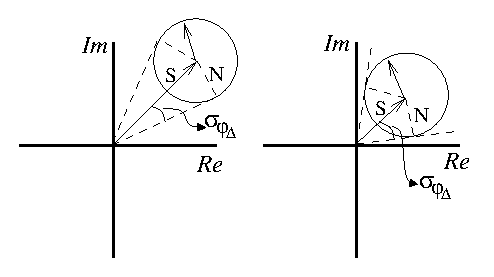
\includegraphics{phasor}% Here is how to import EPS art
\caption{Illustration of closure phase behavior as a function of signal-to-noise ratio in the complex plane. $S$ denotes the true signal amplitude and $N$ the standard deviation from noise. The presence of noise introduces a phase uncertainty, whose standard deviation, $\sigma_{\phi_\Delta}$, is smaller if $S/N$ is larger (left) and vice versa (right). \label{fig:cpphase-cartoon}}
\end{figure}

Eq.~(\ref{eqn:cpphase-sum-sky-noise}) is valid when the gain terms are purely antenna-dependent and in the absence of any dependency on the antenna spacing (also referred to as {\it baseline}). Such terms will be present when mutual coupling across antennas and correlated errors between the signal pathways of the antennas are significant. This will introduce departures from Eq.~(\ref{eqn:cpphase-sum-sky-noise}) that will depend on the magnitude of such effects. In this paper, such baseline-dependent gain terms will be ignored but they will be explored in forthcoming papers describing similar analysis with specific instruments where they may be non-negligible. 

\section{Modeling}\label{sec:modeling}

We describe the instrument and sky model we adopt to demonstrate our approach to EoR H~{\sc i} detection. 

\subsection{Instrument Model}\label{sec:instrument}

We use the Hydrogen Epoch of Reionization Array \cite[HERA;][]{deb17,thy16,ewa16,neb16,patra17} array location, layout \cite{dil16}, and antenna power pattern \cite{deb17} to model the visibilities and bi-spectrum phase. In principle, the HERA layout offers redundant, independent measurements of $\phi_\Delta^\textrm{m}$ for a given class of antenna triplets, which will be discussed in \S\ref{sec:extraction}.

\subsection{Sky Model and Noise}\label{sec:skymodel-noise}

We construct an all-sky model that includes the realization of a fiducial EoR model using 21cmFAST \cite{mes11} and a radio foreground model that includes compact and diffuse synchrotron emission from the Galaxy and extragalactic sources \cite{thy15a}. The models chosen here are only for demonstrating the potential of the technique which will be valid for other models as well.

Fig.~\ref{fig:vis-spectra} shows the amplitudes of the spatial coherence spectra measured at the three 14.6~m antenna spacings comprised of the sky (foreground synchrotron and H~{\sc i} from the EoR) and thermal noise contributions with 1~min integration. It is seen that the foreground contributions exceed the EoR signal by a factor $\sim 10^4$ as expected. It is also noted that $400\lesssim \rho_\textrm{ab},\,\rho_\textrm{bc},\,\rho_\textrm{ca} \lesssim 1600$, which implies that fluctuations in $\phi_\Delta^\textrm{m}$ caused by thermal noise will follow a Gaussian distribution with standard deviation given in Eq.~\ref{eqn:cprms-noise}.

\begin{figure}[htb]
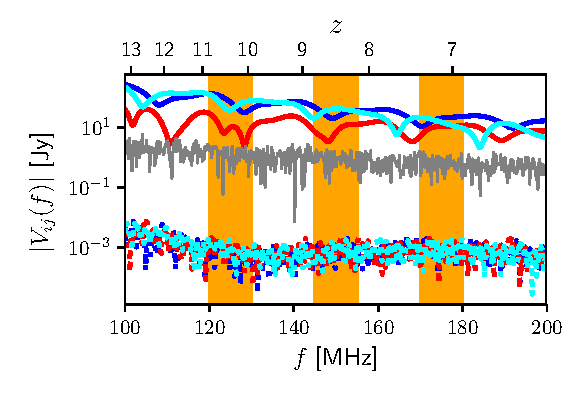
\includegraphics[width=0.85\linewidth]{visamp_spectra_asm_eor_noise}
\caption{Amplitudes of visibility spectra measured on three 14.6~m antenna spacings shown in red, blue and cyan. The black curve shows the typical noise in the measured visibilities obtained with 1~min integration. The solid colored curves show visibility amplitudes from all-sky foreground synchrotron from diffuse and compact components. The dotted curves show the visibility amplitudes from EoR signal on the corresponding antenna spacings from a fiducial model obtained using 21cmFAST. Typically, the EoR signal is $\gtrsim 10^4$ times fainter than the foregrounds. \label{fig:vis-spectra}}
\end{figure}

Fig.~\ref{fig:cp-spectra} shows the spectra of the bi-spectrum phase, $\phi_\Delta$, for the foreground and EoR components separately. It is clearly noted that the foregrounds contributions to $\phi_\Delta$ are characterized by a smooth spectrum while the EoR signal is rapidly fluctuating in comparison. To identify with Eq.~\ref{eqn:cpphase-sum-sky-noise}, we write $\phi_\Delta^\textrm{m}$ as:
\begin{align}\label{eqn:cp-components}
  \phi_\Delta^\textrm{m} &= \left(\phi_\Delta^\textrm{H{\sc i}} + \phi_\Delta^\textrm{F}\right) + \phi_\Delta^\textrm{N}
  % &= \phi_\Delta^\textrm{T} + \phi_\Delta^\textrm{N}, \nonumber
\end{align}
where, the terms in the parenthesis are purely sky-based. 

\begin{figure}[htb]
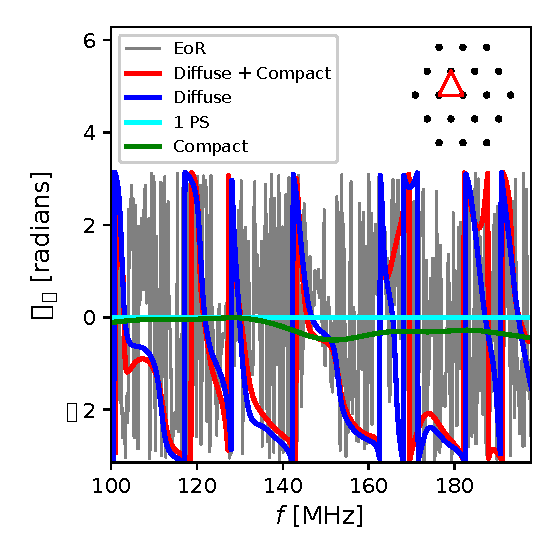
\includegraphics[width=0.85\linewidth]{closure_phase_spectra_1_15_16}
\caption{Closure phase spectra of individual components in the sky model -- single points source (cyan) with $\phi_\Delta=0$, compact sources (green), diffuse foregrounds (blue), all-sky diffuse and compact components combined (red), and the EoR H~{\sc i} fluctuations (gray) -- for an equilateral triad of side 14.6~m in the HERA-19 layout highlighted in the upper right corner. It is seen that the EoR signal is highly fluctuating relative to all the foreground components. \label{fig:cp-spectra}}
\end{figure}

\section{Extraction of the cosmic signal}\label{sec:extraction}

The different spectral characteristics -- smooth $\phi_\Delta^\textrm{F}$ and fluctuating $\phi_\Delta^\textrm{H{\sc i}}$ -- indicate that techniques similar to the power spectrum approaches could be employed to separate the cosmic signal from foregrounds but avoiding the need for high-precision spectral calibration that most other approaches rely on.

If a number of independent samples available, they could be used to average $\phi_\Delta^\textrm{m}$ to reduce the standard deviation of $\phi_\Delta^\textrm{N}$ by taking advantage of its Gaussian distribution, in estimating $\phi_\Delta^\textrm{T}$ with reduced uncertainty. When $\phi_\Delta^\textrm{N}$ is sufficiently low, $\phi_\Delta^\textrm{H{\sc i}}$ will dominate the spectral fluctuations in $\phi_\Delta^\textrm{m}$, while $\phi_\Delta^\textrm{F}$ will be dominant but spectrally smooth. Then the standard deviation in $\phi_\Delta^\textrm{m}$ will be similar in form to Eq.~(\ref{eqn:cprms-noise}):
\begin{align}
  \sigma_{\phi_\Delta^\textrm{m}} &= \frac{1}{\sqrt{2}}\left[\left(\frac{1}{\rho_\textrm{ab}^\textrm{H{\sc i}}}\right)^2 + \left(\frac{1}{\rho_\textrm{bc}^\textrm{H{\sc i}}}\right)^2 + \left(\frac{1}{\rho_\textrm{ca}^\textrm{H{\sc i}}}\right)^2\right]^{1/2}, \label{eqn:cprms-EoR}
\end{align}
where, $\rho_\textrm{ab}^\textrm{H{\sc i}} = |V_\textrm{ab}^\textrm{T}|/|V_\textrm{ab}^\textrm{H{\sc i}}| \approx |V_\textrm{ab}^\textrm{F}|/|V_\textrm{ab}^\textrm{H{\sc i}}|$. Here, $V_\textrm{ab}^\textrm{F}$ denotes the contributions from the foregrounds to the spatial coherence spectrum. This approximation is usually valid because $\rho_\textrm{ab}^\textrm{H{\sc i}} \gg 1$ (expected to be $\sim 10^4$) and $V_\textrm{ab}^\textrm{T} \approx V_\textrm{ab}^\textrm{F}$. 

Thus, when $\rho_\textrm{ab}^\textrm{H{\sc i}} < \rho_\textrm{ab}^\textrm{N}$ is valid, $\sigma_{\phi_\Delta^\textrm{m}}$ can be used to estimate $|V_\textrm{ab}^\textrm{F}|/|V_\textrm{ab}^\textrm{H{\sc i}}|$, which in turn can be used to infer $|V_\textrm{ab}^\textrm{H{\sc i}}|$ if $V_\textrm{ab}^\textrm{F}$ is known. This has a direct bearing on the spin-temperature, $T_{21}$, as a function of frequency, or redshift. The accuracy of this estimate will be set by the uncertainty in the $V_\textrm{ab}^\textrm{F}$ model.

% \subsection{Separability using Delay Spectrum}\label{sec:delay-spectrum}

\subsection{EoR window and Foreground wedge}\label{sec:cp-FG-wedge}

While any method that relies on separating a signal from contaminants using differences in spectral characteristics is applicable, we employ the {\it Delay Spectrum} approach \cite{par12a,par12b} to demonstrate the separability of the EoR signal. Since the $\phi_\Delta$ spectrum can wrap around the boundaries at $\pm\pi$, a Fourier transform of this quantity will introduce non-physical spectral structure. Hence, we define $\xi_\Delta = e^{i\phi_\Delta}$, on which we perform a delay transform as follows:
\begin{align}\label{eqn:cpdspec}
  \Xi_\Delta(\tau) &= \int \xi_\Delta(f)\,W(f)\,e^{i2\pi f\tau}\,\mathrm{d}f,
\end{align}
where, $W(f)$ is a spectral weighting function that can be chosen to control the quality of the delay spectrum \citep{thy13,thy16} and has a width $B_\textrm{eff}$, the effective bandwidth. From Eq.~(\ref{eqn:cpphase-sum-of-visphases}), $\xi_\Delta = e^{i\phi_\textrm{ab}}\,e^{i\phi_\textrm{bc}}\,e^{i\phi_\textrm{ca}}$. Hence,
\begin{align}
  \Xi_\Delta(\tau) &= \Xi_\textrm{ab}(\tau) \star \Xi_\textrm{bc}(\tau) \star \Xi_\textrm{ca}(\tau) \star \mathcal{W}(\tau), \label{eqn:cpdspec-convolution}
\end{align}
where, $\{\xi_\textrm{ab}(f),\,\Xi_\textrm{ab}(\tau)\}$, and $\{W(f),\,\mathcal{W}(\tau)\}$ are delay-transform pairs, and $\star$ denotes convolution. 

% \subsubsection{{\it EoR window} and {\it Foreground wedge}}\label{sec:cp-FG-wedge}

Foreground contributions to spatial coherence are expected to be restricted to a wedge-shaped region in three-dimensional wavenumber ($k$) coordinates \cite{bow09,liu09,liu14a,liu14b,dat10,liu11,gho12,mor12,par12b,tro12,ved12,dil13,pob13,thy13,thy15a,thy15b,thy16,dil14}. The maximum extent along $\tau$ ($\propto k_\parallel$) to which foreground contribution in spatial coherence extends is a direct measure of the fastest spectral variation in the foreground component. This maximum delay is proportional to the spacing between antennas ($\propto k_\perp$) measuring the spatial coherence. This gives rise to the {\it foreground wedge}. Eq.~(\ref{eqn:cpdspec-convolution}) shows that $\Xi_\Delta(\tau)$ results from the convolution of the delay spectrum responses of the phases of spatial coherence of three antenna spacings, $\Xi_\Delta(\tau)$ will also exhibit a corresponding wedge-like behavior corresponding to modes:
\begin{align}
  |\tau_\textrm{F}| \lesssim \frac{|\bm{b}_\textrm{ab}| + |\bm{b}_\textrm{bc}| + |\bm{b}_\textrm{ca}|}{c} + \frac{1}{B_\textrm{eff}}, \label{eqn:cp-FG-wedge}
\end{align}
where, $\bm{b}_\textrm{ab}$, $\bm{b}_\textrm{bc}$, and $\bm{b}_\textrm{ca}$ are the three antenna spacings, and the last term represents the width added by the convolution with $\mathcal{W}(\tau)$. The presence of three antenna spacings makes their correspondence with $k_\perp$ not straightforward unlike in a power spectrum approach. The maximum $k_\parallel$-mode of foreground contamination extends farther than in a power spectrum approach and the {\it EoR window} shrinks  correspondingly along $k_\parallel$. However, the {\it EoR window} still has a finite extent in which the spectral features imprinted by $\phi_\Delta^\textrm{H{\sc i}}$ will dominate and contamination from $\phi_\Delta^\textrm{F}$ will be minimal, in $k_\parallel$-modes corresponding to:
\begin{align}
  |\tau_\textrm{F}| < |\tau| \leq 1/(2\,\Delta f), \label{eqn:cp-EoR-window}
\end{align}
where, $\Delta f$ is the frequency resolution, and $1/(2\,\Delta f)$ denotes the shortest line-of-sight spatial, or largest $k_\parallel$, modes in the measurements.

To use existing definitions, we assign an amplitude of 1~Jy to $\xi_\Delta(f)$ and define its delay cross-power spectrum as \cite{par12a,thy15a}:
\begin{align}
  P_\Delta(k_\parallel) &\equiv \mathfrak{Re}\bigg\{\Xi_\Delta(\tau)\Xi_{\Delta^\prime}^*(\tau)\bigg\} \nonumber\\
  &\quad \times \left(\frac{1}{\Omega B_\textrm{eff}}\right)\left(\frac{D^2\Delta D}{B_\textrm{eff}}\right)\left(\frac{\lambda^2}{2k_\textrm{B}}\right)^2, \label{eqn:delay-power-spectrum}
\end{align}
where, $\mathfrak{Re}\{\cdot\}$ denotes the real part, $B_\textrm{eff}$ is the bandwidth, $\lambda$ is the wavelength of the band center, $k_\textrm{B}$ is the Boltzmann constant, $\boldsymbol{k}_\perp$ and $k_\parallel$ are the transverse (on the sky) and line-of-sight (into the sky) wavenumbers respectively, $f_{21}$ is the rest-frame frequency of the 21~cm spin-flip transition of H{\sc i}, $z$ is the redshift, $D\equiv D(z)$ is the transverse comoving distance, $\Delta D$ is the comoving depth along the line of sight corresponding to $B_\textrm{eff}$, and $h$, $H_0$ and $E(z)\equiv [\Omega_\textrm{M}(1+z)^3+\Omega_\textrm{k}(1+z)^2+\Omega_\Lambda]^{1/2}$ are standard terms in cosmology. In this paper, we use $\Omega_\textrm{M}=0.27$, $\Omega_\Lambda=0.73$, $\Omega_\textrm{K}=1-\Omega_\textrm{M}-\Omega_\Lambda$, $H_0=100\,h\,$km$\,$s$^{-1}\,$Mpc$^{-1}$ \cite{wmap9cosmo}. In the case when $\Xi_\Delta(\tau)$ and $\Xi_{\Delta^\prime}(\tau)$ are identical, $P_\Delta(k_\parallel)$ reduces to delay auto-power spectrum. In \S\ref{sec:averaging}, we describe how Eq.~(\ref{eqn:delay-power-spectrum}) may be used in different contexts. In Eq.~(\ref{eqn:delay-power-spectrum}), $P_\Delta(k_\parallel)$ is in units of K$^2 (h^{-1}$~Mpc$)^3$, but these units are relative since the amplitude of $\xi_\Delta(f)$ was chosen arbitrarily. 

\subsection{Improving S/N in measurements}\label{sec:averaging}

As discussed above, we require $\sigma_{\phi_\Delta^\textrm{H{\sc i}}} > \sigma_{\phi_\Delta^\textrm{N}}$ such that $\phi_\Delta^\textrm{F}, \phi_\Delta^\textrm{H{\sc i}} > \phi_\Delta^\textrm{N}$ in order to detect EoR and estimate $\rho_\textrm{ab}^\textrm{H{\sc i}}$. This can be achieved by a combination of the following.

\subsubsection{Visibility Averaging}\label{sec:vis-avg}

If the antenna gains are known to be stable, uncalibrated spatial coherence can be averaged over a time interval above which the measured spatial coherence becomes incoherent in phase. This coherence timescale is usually determined by field of view and antenna spacing, or characteristic timescale for ionospheric fluctuations and/or instrumental changes, whichever is lesser. Beyond this timescale, the spatial coherence is either intrinsically different or has to be calibrated. This will provide the initial $\rho_\textrm{ab}^\textrm{N}$ and will serve as a basic measurement unit upon which the S/N can be further improved using the following steps. 

\subsubsection{Averaging in local sidereal time from day to day}\label{sec:lst-avg}

Since the visible sky will be identical at the same {\it local sidereal time} (LST) when repeated across multiple days of observation, $\phi_\Delta^\textrm{F}$ and $\phi_\Delta^\textrm{H{\sc i}}$ will remain constant whereas $\phi_\Delta^\textrm{N}$ will be independent across these observations. This allows for coherent averaging of $\phi_\Delta^\textrm{m}$ and reduce the variance due to $\phi_\Delta^\textrm{N}$.

Day-to-day variations in ionosphere will not affect $\phi_\Delta^\textrm{m}$ measured over different days as long as either the instrument has a small field of view or the size of the array is small compared to the predominant spatial scales in the ionospheric variations. For example, this has been observed to be the case for HERA \cite{car18}. In such scenarios, $\phi_\Delta^\textrm{m}$ can be averaged across multiple days at a fixed LST before computing $P_\Delta(k_\parallel)$ in Eq.~(\ref{eqn:delay-power-spectrum}), where $\Xi_\Delta(\tau)=\Xi_{\Delta^\prime}^*(\tau)$. 

\subsubsection{Averaging antenna triads}\label{sec:triad-avg}

Depending on the degree to which different triads of antennas in the interferometer array are similar, the measurements across these triads can be averaged coherently in $\phi_\Delta^\textrm{m}$ or incoherently in $P_\Delta(k_\parallel)$. If the triads are identical, they will measure $\phi_\Delta^\textrm{m}$ identically as well. This will require redundant placement of antennas such as HERA. Non-redundant spacings of antennas or slight dissimilarities between antenna characteristics or position errors even in supposedly redundant arrays will mean $\phi_\Delta^\textrm{m}$ cannot be averaged coherently because $\phi_\Delta^\textrm{F}$ and $\phi_\Delta^\textrm{H{\sc i}}$ will not remain constant across the antenna triads. In such a scenario, if these variations are not completely different, and assuming they are random across the different antenna triads, the effective thermal noise contribution to $P_\Delta(k_\parallel)$ and statistical variations across triads can still be reduced by incoherent averaging where $P_\Delta(k_\parallel)$ is computed for each pair of triads $\Xi_\Delta(\tau)$ and $\Xi_{\Delta^\prime}^*(\tau)$ and then averaged. The improvement in sensitivity from such an operation will not be as effective as an ideally redundant array.

\subsubsection{Averaging contiguous scans}\label{sec:utc-avg}

Measurements spaced in time larger than the coherence timescale in \S\ref{sec:vis-avg} will not be coherent and thus cannot be averaged in $\phi_\Delta^\textrm{m}$. However, since the cosmological EoR signal is statistically isotropic in space while the foregrounds are not, the different measurements can be used to first compute the individual delay cross-power spectra, $P_\Delta(k_\parallel)$ pairwise across all measurements $\Xi_\Delta(\tau)$ and $\Xi_{\Delta^\prime}^*(\tau)$ and then be averaged as described in \S\ref{sec:triad-avg}. This will improve sensitivity by reducing both thermal noise and foreground contributions in $P_\Delta(k_\parallel)$. 

% \section{Discussion}\label{sec:discussion}

\subsection{Detection of Cosmic Reionization}\label{sec:EoR-detection}

One of the primary applications of this technique is to detect EoR. This is generically applicable to any interferometer array. In this paper, we use the following parameters and HERA as an example to demonstrate the potential of this technique.

We consider the spectral band 100--200~MHz divided into 512 spectral channels, each 195.3125~kHz wide. Using a simulated HERA antenna power pattern \cite{deb17}, we used PRISim \footnote{PRISim is the open source Precision Radio Interferometry Simulator Python package available at \href{https://github.com/nithyanandan/PRISim}{https://github.com/nithyanandan/PRISim}.} to simulate the propagation of a sky signal consisting of synchrotron foregrounds and EoR models, and thermal noise as described in \S\ref{sec:modeling} and obtain the spatial coherence spectra, $V_\textrm{ab}^\textrm{T}(f) + V_\textrm{ab}^\textrm{N}(f)$, on various antenna spacings for an integration interval of 1~min, which we consider as the conservative estimate for coherence timescale (see \S\ref{sec:vis-avg}) \cite{car18}. These were shown in Fig.~\ref{fig:vis-spectra}, which indicate $400\lesssim \rho_\textrm{ab}^\textrm{N} \lesssim 1200$ and are in the high S/N regime where $\phi_\textrm{ab}^\textrm{N}$ and $\phi_\Delta^\textrm{N}$ are well approximated by a Gaussian distribution. 

For bi-spectrum phase, we consider antenna triads forming equilateral triangles of side 14.6~m. For simplicity, we assume that all such triads are ideally redundant in $\phi_\Delta^\textrm{m}$, only differing by uncorrelated thermal noise, $\phi_\Delta^\textrm{T}$. We assume that the total number of such available measurements to be $N_\textrm{m} \sim 10^6$. For each of these measurements, $\phi_\Delta^\textrm{N}$ was drawn from a Gaussian distribution using $\sigma_{\phi_\Delta^\textrm{N}}$ in Eq.~(\ref{eqn:cprms-noise}). As various combinations of coherent and incoherent averaging depend on the specific instrument characteristics, we keep this analysis generic by assuming there are $N_\textrm{c}$ coherent measurements of $\phi_\Delta^\textrm{m}$ and for each of these measurements, there are $N_\textrm{ic}$ incoherent measurements such that $N_\textrm{c}N_\textrm{ic}=N_\textrm{m}$. $\phi_\Delta^\textrm{m}$ is averaged coherently over $N_\textrm{c}$ measurements, and then averaged incoherently over $P_\Delta(k_\parallel)$ measured for all non-redundant pairs of $\phi_\Delta^\textrm{m}$. For computing delay spectrum, $\Xi_\Delta(\tau)$, we choose $W(f)$ by applying inverse Fourier transform of the squared delay response of a {\it Blackman-Harris} spectral window \cite{har78} as proposed in \cite{thy16}, using a subband centered at 125~MHz, 150~MHz, and 175~MHz with an effective bandwidth of $B_\textrm{eff}\simeq 10$~MHz in order to minimize EoR signal evolution in the corresponding redshift range.

Fig.~\ref{fig:cpdps} shows the delay power spectrum, $P_\Delta(k_\parallel)$, of $\phi_\Delta^\textrm{m}$ obtained for the subband centered at 150~MHz, a conservative initial S/N, $\rho_\textrm{ab}^\textrm{N}=400$,  for these chosen parameters. The vertical lines show the boundaries of the {\it foreground wedge} (see \S\ref{sec:cp-FG-wedge}, Eq.~(\ref{eqn:cp-FG-wedge})) and the foreground contributions decline drastically beyond these boundaries. In the {\it EoR window} at $|k_\parallel| \gtrsim 0.5\,h$~Mpc$^{-1}$, the contributions from the cosmological H~{\sc i} fluctuations, $\phi_\Delta^\textrm{H{\sc i}}$, dominate over $\phi_\Delta^\textrm{F} + \phi_\Delta^\textrm{N}$. It clearly shows that $N_\textrm{m}$ used in this example is sufficient to make $\rho_\textrm{ab}^\textrm{N} < \rho_\textrm{ab}^\textrm{H{\sc i}}$ and the cosmological H~{\sc i} fluctuations detectable in individual line-of-sight modes, $|k_\parallel| \gtrsim 0.5\,h$~Mpc$^{-1}$. 

\begin{figure}[htb]
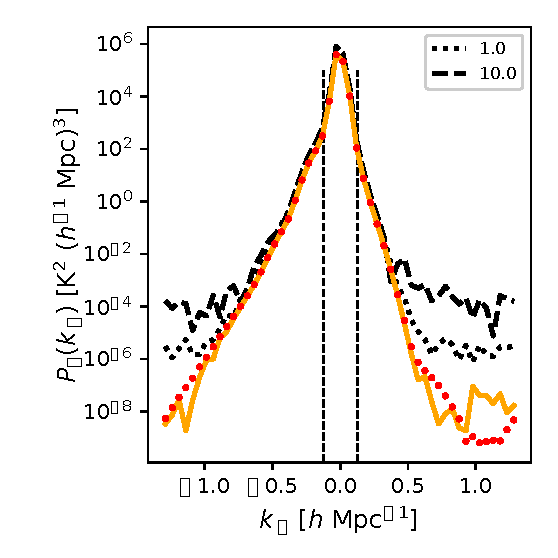
\includegraphics[width=0.85\linewidth]{cpdps_150MHz_nsamples_1048576}
\caption{The delay power spectrum of simulated closure phases that includes contributions from foregrounds, EoR signal, and thermal noise. The vertical dashed black lines denote the boundaries of the {\it foreground wedge} corresponding to Eq.~(\ref{eqn:cp-FG-wedge}). The red curve denotes when only foregrounds are present. The orange curve is for thermal noise superimposed on the foreground component after averaging $\phi_\Delta^\textrm{F}+\phi_\Delta^\textrm{N}$ with $N_\textrm{m} \sim 10^6$ measurements. The black dotted curve is the delay power spectrum when contribution from a fiducial model of EoR is present, $\phi_\Delta^\textrm{m}=\phi_\Delta^\textrm{F}+\phi_\Delta^\textrm{H{\sc i}}+\phi_\Delta^\textrm{N}$, after averaging same number of measurements. The black dashed curve is the same as the black dotted curve except the fiducial EoR model is 10 times stronger in $T_{21}$. It is noted that with sufficient mitigation of thermal noise contributions through averaging independent measurements, the EoR contribution is significantly detectable at $|k_\parallel| \gtrsim 0.5\,h$~Mpc$^{-1}$. The significance of EoR detection depends the strength of $T_{21}$ relative to the foregrounds. An increase in $T_{21}$ by a factor of 10 shows an increase by $\sim 100$ in power spectrum, strongly indicating that it is a sensitive function of $\rho_\textrm{ab}^\textrm{H{\sc i}}$, and thus can be used in inferring $T_{21}(z)$ if a reliable foreground model is available. \label{fig:cpdps}}
\end{figure}

\subsection{Estimation of Spin Temperature from the EoR}\label{sec:spin-temp}

Another primary application of this approach is to estimate the average $T_{21}(z)$ in various subbands using the separation in delay power spectrum, $P_\Delta(k_\parallel)$, demonstrated above. When $\rho_\textrm{ab}^\textrm{H{\sc i}} < \rho_\textrm{ab}^\textrm{N}$, the separation between $\phi_\Delta^\textrm{m}$ and $\phi_\Delta^\textrm{F} + \phi_\Delta^\textrm{N}$ in $P_\Delta(k_\parallel)$ is expected to be a sensitive function of $\rho_\textrm{ab}^\textrm{H{\sc i}}$. Fig.~\ref{fig:cpdps} shows $P_\Delta(k_\parallel)$ for various values of simulated $T_{21}(z)$, or equivalently, $\rho_\textrm{ab}^\textrm{H{\sc i}}$ while keeping the foreground model fixed. It can be seen that as the strength of the EoR H{\sc i} component increases, the separation clearly increases in $P_\Delta(k_\parallel)$ at $|k_\parallel| \gtrsim 0.5\,h$~Mpc$^{-1}$. Conversely, during analysis, based on this separation in delay spectrum, $\rho_\textrm{ab}^\textrm{H{\sc i}}$ can be estimated in the different subbands, or redshift ranges. This can be taken a step further to estimate $T_{21}(z)$ if the foreground model is known in the different subbands. The uncertainty in this estimate will depend on the uncertainty on the foreground model. The easiest confirmation of this hypothesis can be obtained by estimating $\rho_\textrm{ab}^\textrm{H{\sc i}}$ in different subbands and verifying that there is no separation at $|k_\parallel| \gtrsim 0.5\,h$~Mpc$^{-1}$ at $z\lesssim 6$, when EoR is believed to have ended. This will correspond to $(\rho_\textrm{ab}^\textrm{H{\sc i}})^{-1} \ll 1$. Lack of separation in power spectrum will enable placing reliable upper limits on $T_{21}(z)$.

\subsection{Prospects and Challenges}\label{sec:prospects-challenges}

We have presented a simple analysis of the concept behind this new approach. There are a number of ways in which the prospects of detecting EoR can be improved.

\begin{enumerate}
\item The completed layout of HERA will consist of 350 antennas yielding $\sim$~10--100 times more measurements than at present. This will reduce both thermal noise and systematics significantly. 
\item Analysis techniques such as inverse-covariance weighting \cite{liu14a,liu14b,dil15} will be employed in analyzing data to maximize sensitivity.
\item Our analysis demonstrates EoR detection prospects on individual classes of antenna triads ($k_\perp$-modes) and $k_\parallel$-modes. Cylindrical and spherical binning in $k$-modes with optimal weighting, analogous to that employed in power spectrum approaches, will further improve sensitivity compared to the simple demonstration-scale analysis presented here.
\item To reduce the magnitude of continuum (smooth spectrum) power leakage into higher $k_\parallel$-modes, the smooth variation in $\xi_\Delta(f)$ may be removed first before applying Eq.~(\ref{eqn:cpdspec}). This will render $\xi_\Delta(f)$ largely free of foregrounds and further improve the sensitivity. This may also reduce loss of sensitivity caused by radio frequency interference (RFI) by mitigating artificially sharp spectral features (see more discussion below). From this perspective, it will provide significantly higher sensitivity than the conservative approach presented in our work.
\end{enumerate}

We identify the following challenges for this approach.

\begin{enumerate}
\item As described in \S\ref{sec:cp-FG-wedge}, the {\it EoR window} is shrunk in this approach and thus may have smaller number of uncontaminated $k$-modes containing cosmological information. But considering a major systematic arising from antenna-based calibration is avoided, this trade-off may still be desirable.
\item Unlike in power spectrum approach, our approach cannot pre-filter for foreground contributions using delay and fringe rate filtering. This is because they introduce spatial filters on the sky structure that depend on the orientation and length of the antenna spacings and thus the three antenna spacings in $\phi_\Delta^\textrm{m}$ will observe a filtered sky that will not be identical thus invalidating the properties of bi-spectrum phase on which this analysis is based. The presence of bright foreground component may provide a higher $\rho_\textrm{ab}^\textrm{N}$ and thus a lower $\sigma_{\phi_\Delta^\textrm{N}}$, assuming $V_\textrm{ab}^\textrm{N}(f)$ does not depend significantly on the sky. However, our approach without such baseline-dependent filtering in delay and fringe rate has still shown separation of cosmological signal from foregrounds in $k_\parallel$-modes. Further, owing to its simplicity, our approach is not very susceptible to loss of cosmological usually introduced by such filters.
\item Presence of significant baseline-based gain terms will introduce systematic errors in addition to the noise-like terms in Eq.~(\ref{eqn:bispectrum-terms}). If they are small relative to antenna-based gains, they may be treated as additional perturbation terms in Eq.~(\ref{eqn:closure-asymptotic}). If their variation across different antenna spacings are random and/or spectrally smooth, their effects can still be minimized by incoherent averaging described in \S\ref{sec:averaging} though overall sensitivity may have been degraded. This is an issue that will affect current approaches as well. Thus far, such baseline-based gains have not been found to be a significant limiting factor. 
\item Presence of off-diagonal terms in the direction-independent Jones matrix of an antenna indicative of polarization leakage between the dual-polarization feeds of an antenna are still antenna-based and yet will introduce systematic departures from Eq.~(\ref{eqn:bispectrum-terms}). Some of the remedies described above for baseline-based gain terms are applicable for this issue as well. Current approaches are also susceptible to this issue but so far it has not been found to be a dominant limitation.
\item Presence of non-identical antenna beams (power patterns) filters the sky differently for the three components in the triad and thus will introduce departures from expected properties of $\phi_\Delta^\textrm{m}$. These pose a challenge to current approaches as well and some of the proposed remedies may be applicable in this context as well.
\item Flagging of frequency channels affected by radio frequency interference (RFI) will introduce artificially sharp spectral structures which will leak power into higher $k_\parallel$ modes, just as in current power spectrum approaches. Careful spectral interpolation in flagged channels, though cannot recover the cosmological fluctuations in the channels, is found to be promising in recovering the smooth contributions from foreground synchrotron. Algorithms to immunize analysis against RFI that are currently in use for power spectrum approaches may be employed to arrest loss of sensitivity in critical $k_\parallel$ modes. We leave a more thorough investigation of effects of RFI and flagging to future work.
\end{enumerate}

Our approach is generically applicable to non-redundant arrays as well. However, as in current approaches, effects that introduce non-identical behavior in the triad components in general will pose a challenge to this approach and the effectiveness of remedial techniques will depend on the magnitude of these effects. Current HERA, with 47 antennas, in a season of observing will have enough data to either provide preliminary constraints on the EoR if not limited by spectral systematics or clearly indicate the nature of these systematic limitations.

\section{Summary}\label{sec:summary}

Current low-frequency EoR experiments based on redshifted 21~cm measurements are found to be limited by spectral systematics. One of the primary limiting challenges is the need for high-precision spectral calibration. We propose a new approach that uses bi-spectrum phase. It represents an intrinsic property of the sky and is thus impervious to antenna-based calibration, unlike current approaches.
  
We show that it has parallels with current approaches and demonstrate that differences in spectral characteristics of the EoR H~{\sc i} and bright foregrounds in bi-spectrum phase can be used to separate them using a delay-spectrum approach. We note the prospects of detection and EoR model constraints can be further improved in a number of ways relative to the simple analysis presented here. We have listed a number of challenges that may limit this approach while noting that even current approaches are subject to most of these challenges.
  
Data obtained with 47-dish HERA in a single season ($\sim$~150 nights) of observing will have enough information to either detect EoR or indicate clearly what the limitations are using our approach. Analysis of data is underway and will be presented in forthcoming papers.

\begin{acknowledgments}
We wish to acknowledge the insightful discussions with Aaron Parsons, James Aguirre, Rajaram Nityananda, and James Moran that helped significantly in the preparation of this manuscript.
\end{acknowledgments}

% \subsection{\label{sec:level2}Second-level heading: Formatting}

% This file may be formatted in either the \texttt{preprint} or
% \texttt{reprint} style. \texttt{reprint} format mimics final journal output. 
% Either format may be used for submission purposes. \texttt{letter} sized paper should
% be used when submitting to APS journals.

% \subsubsection{Wide text (A level-3 head)}
% The \texttt{widetext} environment will make the text the width of the
% full page, as on page~\pageref{eq:wideeq}. (Note the use the
% \verb+\pageref{#1}+ command to refer to the page number.) 
% \paragraph{Note (Fourth-level head is run in)}
% The width-changing commands only take effect in two-column formatting. 
% There is no effect if text is in a single column.

% \subsection{\label{sec:citeref}Citations and References}
% A citation in text uses the command \verb+\cite{#1}+ or
% \verb+\onlinecite{#1}+ and refers to an entry in the bibliography. 
% An entry in the bibliography is a reference to another document.

% \subsubsection{Citations}
% Because REV\TeX\ uses the \verb+natbib+ package of Patrick Daly, 
% the entire repertoire of commands in that package are available for your document;
% see the \verb+natbib+ documentation for further details. Please note that
% REV\TeX\ requires version 8.31a or later of \verb+natbib+.

% \paragraph{Syntax}
% The argument of \verb+\cite+ may be a single \emph{key}, 
% or may consist of a comma-separated list of keys.
% The citation \emph{key} may contain 
% letters, numbers, the dash (-) character, or the period (.) character. 
% New with natbib 8.3 is an extension to the syntax that allows for 
% a star (*) form and two optional arguments on the citation key itself.
% The syntax of the \verb+\cite+ command is thus (informally stated)
% \begin{quotation}\flushleft\leftskip1em
% \verb+\cite+ \verb+{+ \emph{key} \verb+}+, or\\
% \verb+\cite+ \verb+{+ \emph{optarg+key} \verb+}+, or\\
% \verb+\cite+ \verb+{+ \emph{optarg+key} \verb+,+ \emph{optarg+key}\ldots \verb+}+,
% \end{quotation}\noindent
% where \emph{optarg+key} signifies 
% \begin{quotation}\flushleft\leftskip1em
% \emph{key}, or\\
% \texttt{*}\emph{key}, or\\
% \texttt{[}\emph{pre}\texttt{]}\emph{key}, or\\
% \texttt{[}\emph{pre}\texttt{]}\texttt{[}\emph{post}\texttt{]}\emph{key}, or even\\
% \texttt{*}\texttt{[}\emph{pre}\texttt{]}\texttt{[}\emph{post}\texttt{]}\emph{key}.
% \end{quotation}\noindent
% where \emph{pre} and \emph{post} is whatever text you wish to place 
% at the beginning and end, respectively, of the bibliographic reference
% (see Ref.~[\onlinecite{witten2001}] and the two under Ref.~[\onlinecite{feyn54}]).
% (Keep in mind that no automatic space or punctuation is applied.)
% It is highly recommended that you put the entire \emph{pre} or \emph{post} portion 
% within its own set of braces, for example: 
% \verb+\cite+ \verb+{+ \texttt{[} \verb+{+\emph{text}\verb+}+\texttt{]}\emph{key}\verb+}+.
% The extra set of braces will keep \LaTeX\ out of trouble if your \emph{text} contains the comma (,) character.

% The star (*) modifier to the \emph{key} signifies that the reference is to be 
% merged with the previous reference into a single bibliographic entry, 
% a common idiom in APS and AIP articles (see below, Ref.~[\onlinecite{epr}]). 
% When references are merged in this way, they are separated by a semicolon instead of 
% the period (full stop) that would otherwise appear.

% \paragraph{Eliding repeated information}
% When a reference is merged, some of its fields may be elided: for example, 
% when the author matches that of the previous reference, it is omitted. 
% If both author and journal match, both are omitted.
% If the journal matches, but the author does not, the journal is replaced by \emph{ibid.},
% as exemplified by Ref.~[\onlinecite{epr}]. 
% These rules embody common editorial practice in APS and AIP journals and will only
% be in effect if the markup features of the APS and AIP Bib\TeX\ styles is employed.

% \paragraph{The options of the cite command itself}
% Please note that optional arguments to the \emph{key} change the reference in the bibliography, 
% not the citation in the body of the document. 
% For the latter, use the optional arguments of the \verb+\cite+ command itself:
% \verb+\cite+ \texttt{*}\allowbreak
% \texttt{[}\emph{pre-cite}\texttt{]}\allowbreak
% \texttt{[}\emph{post-cite}\texttt{]}\allowbreak
% \verb+{+\emph{key-list}\verb+}+.

% \subsubsection{Example citations}
% By default, citations are numerical\cite{Beutler1994}.
% Author-year citations are used when the journal is RMP. 
% To give a textual citation, use \verb+\onlinecite{#1}+: 
% Refs.~\onlinecite{[][{, and references therein}]witten2001,Bire82}. 
% By default, the \texttt{natbib} package automatically sorts your citations into numerical order and ``compresses'' runs of three or more consecutive numerical citations.
% REV\TeX\ provides the ability to automatically change the punctuation when switching between journal styles that provide citations in square brackets and those that use a superscript style instead. This is done through the \texttt{citeautoscript} option. For instance, the journal style \texttt{prb} automatically invokes this option because \textit{Physical 
% Review B} uses superscript-style citations. The effect is to move the punctuation, which normally comes after a citation in square brackets, to its proper position before the superscript. 
% To illustrate, we cite several together 
% \cite{[See the explanation of time travel in ]feyn54,*[The classical relativistic treatment of ][ is a relative classic]epr,witten2001,Berman1983,Davies1998,Bire82}, 
% and once again in different order (Refs.~\cite{epr,feyn54,Bire82,Berman1983,witten2001,Davies1998}). 
% Note that the citations were both compressed and sorted. Futhermore, running this sample file under the \texttt{prb} option will move the punctuation to the correct place.

% When the \verb+prb+ class option is used, the \verb+\cite{#1}+ command
% displays the reference's number as a superscript rather than in
% square brackets. Note that the location of the \verb+\cite{#1}+
% command should be adjusted for the reference style: the superscript
% references in \verb+prb+ style must appear after punctuation;
% otherwise the reference must appear before any punctuation. This
% sample was written for the regular (non-\texttt{prb}) citation style.
% The command \verb+\onlinecite{#1}+ in the \texttt{prb} style also
% displays the reference on the baseline.

% \subsubsection{References}
% A reference in the bibliography is specified by a \verb+\bibitem{#1}+ command
% with the same argument as the \verb+\cite{#1}+ command.
% \verb+\bibitem{#1}+ commands may be crafted by hand or, preferably,
% generated by Bib\TeX. 
% REV\TeX~4.1 includes Bib\TeX\ style files
% \verb+apsrev4-1.bst+, \verb+apsrmp4-1.bst+ appropriate for
% \textit{Physical Review} and \textit{Reviews of Modern Physics},
% respectively. To display titles for cited journal articles, use the \texttt{longbibliography} class option.

% \subsubsection{Example references}
% This sample file employs the \verb+\bibliography+ command, 
% which formats the \texttt{\jobname .bbl} file
% and specifies which bibliographic databases are to be used by Bib\TeX\ 
% (one of these should be by arXiv convention \texttt{\jobname .bib}).
% Running Bib\TeX\ (via \texttt{bibtex \jobname}) 
% after the first pass of \LaTeX\ produces the file
% \texttt{\jobname .bbl} which contains the automatically formatted
% \verb+\bibitem+ commands (including extra markup information via
% \verb+\bibinfo+ and \verb+\bibfield+ commands). 
% If not using Bib\TeX, you will have to create the \verb+thebibiliography+ environment 
% and its \verb+\bibitem+ commands by hand.

% Numerous examples of the use of the APS bibliographic entry types appear in the bibliography of this sample document.
% You can refer to the \texttt{\jobname .bib} file, 
% and compare its information to the formatted bibliography itself.

% \subsection{Footnotes}%
% Footnotes, produced using the \verb+\footnote{#1}+ command, 
% usually integrated into the bibliography alongside the other entries.
% Numerical citation styles do this%
% \footnote{Automatically placing footnotes into the bibliography requires using BibTeX to compile the bibliography.};
% author-year citation styles place the footnote at the bottom of the text column.
% Note: due to the method used to place footnotes in the bibliography, 
% \emph{you must re-run Bib\TeX\ every time you change any of your document's footnotes}. 

% \section{Math and Equations}
% Inline math may be typeset using the \verb+$+ delimiters. Bold math
% symbols may be achieved using the \verb+bm+ package and the
% \verb+\bm{#1}+ command it supplies. For instance, a bold $\alpha$ can
% be typeset as \verb+$\bm{\alpha}$+ giving $\bm{\alpha}$. Fraktur and
% Blackboard (or open face or double struck) characters should be
% typeset using the \verb+\mathfrak{#1}+ and \verb+\mathbb{#1}+ commands
% respectively. Both are supplied by the \texttt{amssymb} package. For
% example, \verb+$\mathbb{R}$+ gives $\mathbb{R}$ and
% \verb+$\mathfrak{G}$+ gives $\mathfrak{G}$

% In \LaTeX\ there are many different ways to display equations, and a
% few preferred ways are noted below. Displayed math will center by
% default. Use the class option \verb+fleqn+ to flush equations left.

% Below we have numbered single-line equations; this is the most common
% type of equation in \textit{Physical Review}:
% \begin{eqnarray}
% \chi_+(p)\alt{\bf [}2|{\bf p}|(|{\bf p}|+p_z){\bf ]}^{-1/2}
% \left(
% \begin{array}{c}
% |{\bf p}|+p_z\\
% px+ip_y
% \end{array}\right)\;,
% \\
% \left\{%
%  \openone234567890abc123\alpha\beta\gamma\delta1234556\alpha\beta
%  \frac{1\sum^{a}_{b}}{A^2}%
% \right\}%
% \label{eq:one}.
% \end{eqnarray}
% Note the open one in Eq.~(\ref{eq:one}).

% Not all numbered equations will fit within a narrow column this
% way. The equation number will move down automatically if it cannot fit
% on the same line with a one-line equation:
% \begin{equation}
% \left\{
%  ab12345678abc123456abcdef\alpha\beta\gamma\delta1234556\alpha\beta
%  \frac{1\sum^{a}_{b}}{A^2}%
% \right\}.
% \end{equation}

% When the \verb+\label{#1}+ command is used [cf. input for
% Eq.~(\ref{eq:one})], the equation can be referred to in text without
% knowing the equation number that \TeX\ will assign to it. Just
% use \verb+\ref{#1}+, where \verb+#1+ is the same name that used in
% the \verb+\label{#1}+ command.

% Unnumbered single-line equations can be typeset
% using the \verb+\[+, \verb+\]+ format:
% \[g^+g^+ \rightarrow g^+g^+g^+g^+ \dots ~,~~q^+q^+\rightarrow
% q^+g^+g^+ \dots ~. \]


% \subsection{Multiline equations}

% Multiline equations are obtained by using the \verb+eqnarray+
% environment.  Use the \verb+\nonumber+ command at the end of each line
% to avoid assigning a number:
% \begin{eqnarray}
% {\cal M}=&&ig_Z^2(4E_1E_2)^{1/2}(l_i^2)^{-1}
% \delta_{\sigma_1,-\sigma_2}
% (g_{\sigma_2}^e)^2\chi_{-\sigma_2}(p_2)\nonumber\\
% &&\times
% [\epsilon_jl_i\epsilon_i]_{\sigma_1}\chi_{\sigma_1}(p_1),
% \end{eqnarray}
% \begin{eqnarray}
% \sum \vert M^{\text{viol}}_g \vert ^2&=&g^{2n-4}_S(Q^2)~N^{n-2}
%         (N^2-1)\nonumber \\
%  & &\times \left( \sum_{i<j}\right)
%   \sum_{\text{perm}}
%  \frac{1}{S_{12}}
%  \frac{1}{S_{12}}
%  \sum_\tau c^f_\tau~.
% \end{eqnarray}
% \textbf{Note:} Do not use \verb+\label{#1}+ on a line of a multiline
% equation if \verb+\nonumber+ is also used on that line. Incorrect
% cross-referencing will result. Notice the use \verb+\text{#1}+ for
% using a Roman font within a math environment.

% To set a multiline equation without \emph{any} equation
% numbers, use the \verb+\begin{eqnarray*}+,
% \verb+\end{eqnarray*}+ format:
% \begin{eqnarray*}
% \sum \vert M^{\text{viol}}_g \vert ^2&=&g^{2n-4}_S(Q^2)~N^{n-2}
%         (N^2-1)\\
%  & &\times \left( \sum_{i<j}\right)
%  \left(
%   \sum_{\text{perm}}\frac{1}{S_{12}S_{23}S_{n1}}
%  \right)
%  \frac{1}{S_{12}}~.
% \end{eqnarray*}

% To obtain numbers not normally produced by the automatic numbering,
% use the \verb+\tag{#1}+ command, where \verb+#1+ is the desired
% equation number. For example, to get an equation number of
% (\ref{eq:mynum}),
% \begin{equation}
% g^+g^+ \rightarrow g^+g^+g^+g^+ \dots ~,~~q^+q^+\rightarrow
% q^+g^+g^+ \dots ~. \tag{2.6$'$}\label{eq:mynum}
% \end{equation}

% \paragraph{A few notes on \texttt{tag}s} 
% \verb+\tag{#1}+ requires the \texttt{amsmath} package. 
% Place the \verb+\tag{#1}+ command before the \verb+\label{#1}+, if any. 
% The numbering produced by \verb+\tag{#1}+ \textit{does not affect} 
% the automatic numbering in REV\TeX; 
% therefore, the number must be known ahead of time, 
% and it must be manually adjusted if other equations are added. 
% \verb+\tag{#1}+ works with both single-line and multiline equations. 
% \verb+\tag{#1}+ should only be used in exceptional cases---%
% do not use it to number many equations in your paper. 
% Please note that this feature of the \texttt{amsmath} package
% is \emph{not} compatible with the \texttt{hyperref} (6.77u) package.

% Enclosing display math within
% \verb+\begin{subequations}+ and \verb+\end{subequations}+ will produce
% a set of equations that are labeled with letters, as shown in
% Eqs.~(\ref{subeq:1}) and (\ref{subeq:2}) below.
% You may include any number of single-line and multiline equations,
% although it is probably not a good idea to follow one display math
% directly after another.
% \begin{subequations}
% \label{eq:whole}
% \begin{eqnarray}
% {\cal M}=&&ig_Z^2(4E_1E_2)^{1/2}(l_i^2)^{-1}
% (g_{\sigma_2}^e)^2\chi_{-\sigma_2}(p_2)\nonumber\\
% &&\times
% [\epsilon_i]_{\sigma_1}\chi_{\sigma_1}(p_1).\label{subeq:2}
% \end{eqnarray}
% \begin{equation}
% \left\{
%  abc123456abcdef\alpha\beta\gamma\delta1234556\alpha\beta
%  \frac{1\sum^{a}_{b}}{A^2}
% \right\},\label{subeq:1}
% \end{equation}
% \end{subequations}
% Giving a \verb+\label{#1}+ command directly after the \verb+\begin{subequations}+, 
% allows you to reference all the equations in the \texttt{subequations} environment. 
% For example, the equations in the preceding subequations environment were
% Eqs.~(\ref{eq:whole}).

% \subsubsection{Wide equations}
% The equation that follows is set in a wide format, i.e., it spans the full page. 
% The wide format is reserved for long equations
% that cannot easily be set in a single column:
% \begin{widetext}
% \begin{equation}
% {\cal R}^{(\text{d})}=
%  g_{\sigma_2}^e
%  \left(
%    \frac{[\Gamma^Z(3,21)]_{\sigma_1}}{Q_{12}^2-M_W^2}
%   +\frac{[\Gamma^Z(13,2)]_{\sigma_1}}{Q_{13}^2-M_W^2}
%  \right)
%  + x_WQ_e
%  \left(
%    \frac{[\Gamma^\gamma(3,21)]_{\sigma_1}}{Q_{12}^2-M_W^2}
%   +\frac{[\Gamma^\gamma(13,2)]_{\sigma_1}}{Q_{13}^2-M_W^2}
%  \right)\;. 
%  \label{eq:wideeq}
% \end{equation}
% \end{widetext}
% This is typed to show how the output appears in wide format.
% (Incidentally, since there is no blank line between the \texttt{equation} environment above 
% and the start of this paragraph, this paragraph is not indented.)

% \section{Cross-referencing}
% REV\TeX{} will automatically number such things as
% sections, footnotes, equations, figure captions, and table captions. 
% In order to reference them in text, use the
% \verb+\label{#1}+ and \verb+\ref{#1}+ commands. 
% To reference a particular page, use the \verb+\pageref{#1}+ command.

% The \verb+\label{#1}+ should appear 
% within the section heading, 
% within the footnote text, 
% within the equation, or 
% within the table or figure caption. 
% The \verb+\ref{#1}+ command
% is used in text at the point where the reference is to be displayed.  
% Some examples: Section~\ref{sec:level1} on page~\pageref{sec:level1},
% Table~\ref{tab:table1},%
% \begin{table}[b]%The best place to locate the table environment is directly after its first reference in text
% \caption{\label{tab:table1}%
% A table that fits into a single column of a two-column layout. 
% Note that REV\TeX~4 adjusts the intercolumn spacing so that the table fills the
% entire width of the column. Table captions are numbered
% automatically. 
% This table illustrates left-, center-, decimal- and right-aligned columns,
% along with the use of the \texttt{ruledtabular} environment which sets the 
% Scotch (double) rules above and below the alignment, per APS style.
% }
% \begin{ruledtabular}
% \begin{tabular}{lcdr}
% \textrm{Left\footnote{Note a.}}&
% \textrm{Centered\footnote{Note b.}}&
% \multicolumn{1}{c}{\textrm{Decimal}}&
% \textrm{Right}\\
% \colrule
% 1 & 2 & 3.001 & 4\\
% 10 & 20 & 30 & 40\\
% 100 & 200 & 300.0 & 400\\
% \end{tabular}
% \end{ruledtabular}
% \end{table}
% and Fig.~\ref{fig:epsart}.%
% \begin{figure}[b]
% \includegraphics{fig_1}% Here is how to import EPS art
% \caption{\label{fig:epsart} A figure caption. The figure captions are
% automatically numbered.}
% \end{figure}

% \section{Floats: Figures, Tables, Videos, etc.}
% Figures and tables are usually allowed to ``float'', which means that their
% placement is determined by \LaTeX, while the document is being typeset. 

% Use the \texttt{figure} environment for a figure, the \texttt{table} environment for a table.
% In each case, use the \verb+\caption+ command within to give the text of the
% figure or table caption along with the \verb+\label+ command to provide
% a key for referring to this figure or table.
% The typical content of a figure is an image of some kind; 
% that of a table is an alignment.%
% \begin{figure*}
% \includegraphics{fig_2}% Here is how to import EPS art
% \caption{\label{fig:wide}Use the figure* environment to get a wide
% figure that spans the page in \texttt{twocolumn} formatting.}
% \end{figure*}
% \begin{table*}
% \caption{\label{tab:table3}This is a wide table that spans the full page
% width in a two-column layout. It is formatted using the
% \texttt{table*} environment. It also demonstates the use of
% \textbackslash\texttt{multicolumn} in rows with entries that span
% more than one column.}
% \begin{ruledtabular}
% \begin{tabular}{ccccc}
%  &\multicolumn{2}{c}{$D_{4h}^1$}&\multicolumn{2}{c}{$D_{4h}^5$}\\
%  Ion&1st alternative&2nd alternative&lst alternative
% &2nd alternative\\ \hline
%  K&$(2e)+(2f)$&$(4i)$ &$(2c)+(2d)$&$(4f)$ \\
%  Mn&$(2g)$\footnote{The $z$ parameter of these positions is $z\sim\frac{1}{4}$.}
%  &$(a)+(b)+(c)+(d)$&$(4e)$&$(2a)+(2b)$\\
%  Cl&$(a)+(b)+(c)+(d)$&$(2g)$\footnotemark[1]
%  &$(4e)^{\text{a}}$\\
%  He&$(8r)^{\text{a}}$&$(4j)^{\text{a}}$&$(4g)^{\text{a}}$\\
%  Ag& &$(4k)^{\text{a}}$& &$(4h)^{\text{a}}$\\
% \end{tabular}
% \end{ruledtabular}
% \end{table*}

% Insert an image using either the \texttt{graphics} or
% \texttt{graphix} packages, which define the \verb+\includegraphics{#1}+ command.
% (The two packages differ in respect of the optional arguments 
% used to specify the orientation, scaling, and translation of the image.) 
% To create an alignment, use the \texttt{tabular} environment. 

% The best place to locate the \texttt{figure} or \texttt{table} environment
% is immediately following its first reference in text; this sample document
% illustrates this practice for Fig.~\ref{fig:epsart}, which
% shows a figure that is small enough to fit in a single column. 

% In exceptional cases, you will need to move the float earlier in the document, as was done
% with Table~\ref{tab:table3}: \LaTeX's float placement algorithms need to know
% about a full-page-width float earlier. 

% Fig.~\ref{fig:wide}
% has content that is too wide for a single column,
% so the \texttt{figure*} environment has been used.%
% \begin{table}[b]
% \caption{\label{tab:table4}%
% Numbers in columns Three--Five are aligned with the ``d'' column specifier 
% (requires the \texttt{dcolumn} package). 
% Non-numeric entries (those entries without a ``.'') in a ``d'' column are aligned on the decimal point. 
% Use the ``D'' specifier for more complex layouts. }
% \begin{ruledtabular}
% \begin{tabular}{ccddd}
% One&Two&
% \multicolumn{1}{c}{\textrm{Three}}&
% \multicolumn{1}{c}{\textrm{Four}}&
% \multicolumn{1}{c}{\textrm{Five}}\\
% %\mbox{Three}&\mbox{Four}&\mbox{Five}\\
% \hline
% one&two&\mbox{three}&\mbox{four}&\mbox{five}\\
% He&2& 2.77234 & 45672. & 0.69 \\
% C\footnote{Some tables require footnotes.}
%   &C\footnote{Some tables need more than one footnote.}
%   & 12537.64 & 37.66345 & 86.37 \\
% \end{tabular}
% \end{ruledtabular}
% \end{table}

% The content of a table is typically a \texttt{tabular} environment, 
% giving rows of type in aligned columns. 
% Column entries separated by \verb+&+'s, and 
% each row ends with \textbackslash\textbackslash. 
% The required argument for the \texttt{tabular} environment
% specifies how data are aligned in the columns. 
% For instance, entries may be centered, left-justified, right-justified, aligned on a decimal
% point. 
% Extra column-spacing may be be specified as well, 
% although REV\TeX~4 sets this spacing so that the columns fill the width of the
% table. Horizontal rules are typeset using the \verb+\hline+
% command. The doubled (or Scotch) rules that appear at the top and
% bottom of a table can be achieved enclosing the \texttt{tabular}
% environment within a \texttt{ruledtabular} environment. Rows whose
% columns span multiple columns can be typeset using the
% \verb+\multicolumn{#1}{#2}{#3}+ command (for example, see the first
% row of Table~\ref{tab:table3}).%

% Tables~\ref{tab:table1}, \ref{tab:table3}, \ref{tab:table4}, and \ref{tab:table2}%
% \begin{table}[b]
% \caption{\label{tab:table2}
% A table with numerous columns that still fits into a single column. 
% Here, several entries share the same footnote. 
% Inspect the \LaTeX\ input for this table to see exactly how it is done.}
% \begin{ruledtabular}
% \begin{tabular}{cccccccc}
%  &$r_c$ (\AA)&$r_0$ (\AA)&$\kappa r_0$&
%  &$r_c$ (\AA) &$r_0$ (\AA)&$\kappa r_0$\\
% \hline
% Cu& 0.800 & 14.10 & 2.550 &Sn\footnotemark[1]
% & 0.680 & 1.870 & 3.700 \\
% Ag& 0.990 & 15.90 & 2.710 &Pb\footnotemark[2]
% & 0.450 & 1.930 & 3.760 \\
% Au& 1.150 & 15.90 & 2.710 &Ca\footnotemark[3]
% & 0.750 & 2.170 & 3.560 \\
% Mg& 0.490 & 17.60 & 3.200 &Sr\footnotemark[4]
% & 0.900 & 2.370 & 3.720 \\
% Zn& 0.300 & 15.20 & 2.970 &Li\footnotemark[2]
% & 0.380 & 1.730 & 2.830 \\
% Cd& 0.530 & 17.10 & 3.160 &Na\footnotemark[5]
% & 0.760 & 2.110 & 3.120 \\
% Hg& 0.550 & 17.80 & 3.220 &K\footnotemark[5]
% &  1.120 & 2.620 & 3.480 \\
% Al& 0.230 & 15.80 & 3.240 &Rb\footnotemark[3]
% & 1.330 & 2.800 & 3.590 \\
% Ga& 0.310 & 16.70 & 3.330 &Cs\footnotemark[4]
% & 1.420 & 3.030 & 3.740 \\
% In& 0.460 & 18.40 & 3.500 &Ba\footnotemark[5]
% & 0.960 & 2.460 & 3.780 \\
% Tl& 0.480 & 18.90 & 3.550 & & & & \\
% \end{tabular}
% \end{ruledtabular}
% \footnotetext[1]{Here's the first, from Ref.~\onlinecite{feyn54}.}
% \footnotetext[2]{Here's the second.}
% \footnotetext[3]{Here's the third.}
% \footnotetext[4]{Here's the fourth.}
% \footnotetext[5]{And etc.}
% \end{table}
% show various effects.
% A table that fits in a single column employs the \texttt{table}
% environment. 
% Table~\ref{tab:table3} is a wide table, set with the \texttt{table*} environment. 
% Long tables may need to break across pages. 
% The most straightforward way to accomplish this is to specify
% the \verb+[H]+ float placement on the \texttt{table} or
% \texttt{table*} environment. 
% However, the \LaTeXe\ package \texttt{longtable} allows headers and footers to be specified for each page of the table. 
% A simple example of the use of \texttt{longtable} can be found
% in the file \texttt{summary.tex} that is included with the REV\TeX~4
% distribution.

% There are two methods for setting footnotes within a table (these
% footnotes will be displayed directly below the table rather than at
% the bottom of the page or in the bibliography). The easiest
% and preferred method is just to use the \verb+\footnote{#1}+
% command. This will automatically enumerate the footnotes with
% lowercase roman letters. However, it is sometimes necessary to have
% multiple entries in the table share the same footnote. In this case,
% there is no choice but to manually create the footnotes using
% \verb+\footnotemark[#1]+ and \verb+\footnotetext[#1]{#2}+.
% \texttt{\#1} is a numeric value. Each time the same value for
% \texttt{\#1} is used, the same mark is produced in the table. The
% \verb+\footnotetext[#1]{#2}+ commands are placed after the \texttt{tabular}
% environment. Examine the \LaTeX\ source and output for
% Tables~\ref{tab:table1} and \ref{tab:table2}
% for examples.

% Video~\ref{vid:PRSTPER.4.010101} 
% illustrates several features new with REV\TeX4.1,
% starting with the \texttt{video} environment, which is in the same category with
% \texttt{figure} and \texttt{table}.%
% \begin{video}
% \href{http://prst-per.aps.org/multimedia/PRSTPER/v4/i1/e010101/e010101_vid1a.mpg}{\includegraphics{vid_1a}}%
%  \quad
% \href{http://prst-per.aps.org/multimedia/PRSTPER/v4/i1/e010101/e010101_vid1b.mpg}{\includegraphics{vid_1b}}
%  \setfloatlink{http://link.aps.org/multimedia/PRSTPER/v4/i1/e010101}%
%  \caption{\label{vid:PRSTPER.4.010101}%
%   Students explain their initial idea about Newton's third law to a teaching assistant. 
%   Clip (a): same force.
%   Clip (b): move backwards.
%  }%
% \end{video}
% The \verb+\setfloatlink+ command causes the title of the video to be a hyperlink to the
% indicated URL; it may be used with any environment that takes the \verb+\caption+
% command.
% The \verb+\href+ command has the same significance as it does in the context of
% the \texttt{hyperref} package: the second argument is a piece of text to be 
% typeset in your document; the first is its hyperlink, a URL.

% \textit{Physical Review} style requires that the initial citation of
% figures or tables be in numerical order in text, so don't cite
% Fig.~\ref{fig:wide} until Fig.~\ref{fig:epsart} has been cited.

% \begin{acknowledgments}
% We wish to acknowledge the support of the author community in using
% REV\TeX{}, offering suggestions and encouragement, testing new versions,
% \dots.
% \end{acknowledgments}

% \appendix

% \section{Appendixes}

% To start the appendixes, use the \verb+\appendix+ command.
% This signals that all following section commands refer to appendixes
% instead of regular sections. Therefore, the \verb+\appendix+ command
% should be used only once---to setup the section commands to act as
% appendixes. Thereafter normal section commands are used. The heading
% for a section can be left empty. For example,
% \begin{verbatim}
% \appendix
% \section{}
% \end{verbatim}
% will produce an appendix heading that says ``APPENDIX A'' and
% \begin{verbatim}
% \appendix
% \section{Background}
% \end{verbatim}
% will produce an appendix heading that says ``APPENDIX A: BACKGROUND''
% (note that the colon is set automatically).

% If there is only one appendix, then the letter ``A'' should not
% appear. This is suppressed by using the star version of the appendix
% command (\verb+\appendix*+ in the place of \verb+\appendix+).

% \section{A little more on appendixes}

% Observe that this appendix was started by using
% \begin{verbatim}
% \section{A little more on appendixes}
% \end{verbatim}

% Note the equation number in an appendix:
% \begin{equation}
% E=mc^2.
% \end{equation}

% \subsection{\label{app:subsec}A subsection in an appendix}

% You can use a subsection or subsubsection in an appendix. Note the
% numbering: we are now in Appendix~\ref{app:subsec}.

% Note the equation numbers in this appendix, produced with the
% subequations environment:
% \begin{subequations}
% \begin{eqnarray}
% E&=&mc, \label{appa}
% \\
% E&=&mc^2, \label{appb}
% \\
% E&\agt& mc^3. \label{appc}
% \end{eqnarray}
% \end{subequations}
% They turn out to be Eqs.~(\ref{appa}), (\ref{appb}), and (\ref{appc}).

% % The \nocite command causes all entries in a bibliography to be printed out
% % whether or not they are actually referenced in the text. This is appropriate
% % for the sample file to show the different styles of references, but authors
% % most likely will not want to use it.
% \nocite{*}

% \bibliography{apssamp}% Produces the bibliography via BibTeX.

\bibliography{eor}% Produces the bibliography via BibTeX.

\end{document}
%
% ****** End of file apssamp.tex ******
